%!TeX root = ../main.tex
% Add the above to each chapter to make compiling the PDF easier in some editors.

\chapter{Background}\label{chapter:Background}

\section{HPC}

High-performance computing, abbreviated as HPC, leverages the compute capacity of supercomputers or computer clusters to solve problems that are highly complex in nature~\cite{ibm_what_2022}. A computer cluster consists of many different computers (nodes) that are interconnected with high-speed, low-latency interconnects. Each node contains a set of similar components a desktop or laptop PC would contain, such as a CPU, RAM, and storage~\cite{iowa_state_university_what_2020}. It should be noted that modern CPUs, especially ones utilized in HPC applications, usually contain multiple physical cores and multiple hardware threads to enable some amount of parallel processing. [example maybe?] Some nodes, just like some PCs, also have a dedicated graphics processing unit (GPU) to accelerate certain types of workloads~\cite{iowa_state_university_what_2020}.
 
  
 [question: does this suffice in 'bridging the gap'?]
 
 
 \section{Graphics Processing Units}
 
 
 \subsection{What are GPUs}
 To begin with, it should be noted that the term graphics processing unit (GPU) does not equate to a graphics card. GPUs are specialized processing units primarily designed for parallel processing and accelerating workloads that require parallel processing ~\cite{intel_what_2022}. A graphics card, on the other hand, is the add-in card that features a PCI-Express link to facilitate communication between CPU and GPU, dedicated memory and power delivery for the GPU, and the GPU itself. It should also be noted that the graphics card usually has its own dedicated PCB. [does this need citing? - more or less common knowledge?] There are also integrated GPUs, which can be embedded alongside the CPU.  These integrated GPUs are usually less powerful compared to discrete GPUs ~\cite{intel_what_2022}.

 \subsection{Uses of GPUs}
 
 GPUs originally began as, as their names suggest, dedicated graphics accelerators optimized for floating-point operations, which are essential to 3D graphics rendering. They were initially developed as a hardware pipeline with fixed functionality, namely to render graphics. Over the years, GPU architecture has evolved from essentially being an integrated frame buffer into a set of general-purpose, highly parallel, programmable processing cores, enabling more general-purpose computation~\cite{mcclanahan_history_2010}. Today, a GPU is more of an accelerator for many different use-cases and workloads. Examples for personal use include gaming, video editing, and content creation~\cite{intel_what_2022}. On the scientific side, GPUs are frequently used to accelerate workloads that require parallel computing, such as machine learning, fluid dynamics, and data science~\cite{nvidia_cuda_2017}.
 
 
 \subsection{GPU Memory}
 Addressing GPU memory, assuming that the GPU is connected via PCI-Express and has its own dedicated video memory, works in the same way as addressing memory in other PCIe devices, which will be briefly touched upon in section \ref{sec:memory}. However, GPU memory usually has higher throughput bandwidths compared to conventional RAM of a similar period. [todo: needs citation, where to find?] As example, current top of the line graphics cards from Nvidia are equipped with GDDR6X memory, which has a theoretical maximum system bandwidth of one terabyte per second.~\cite{nvidia_nvidia_2020, micron_technology_inc_gddr6x_2022} On the other hand, state of the art main memory, currently DDR4, is limited to a bandwidth of about 35 gigabytes per second~\cite{micron_technology_inc_ram_2022}.
 
 [TODO: DDR5 standard, however: numbers hard to find. what to put?]
 
 
 \section{CUDA}
 As GPUs evolved into more general-purpose processing units over the years, there has been a growing need for an application programming interface (API) that enables general-purpose programming on GPUs.
 
 CUDA is a closed source API developed and maintained by Nvidia for general-purpose GPU computing for their GPUs and graphics cards. It is designed to work with C++ and Fortran and comes with a set of GPU-accelerated libraries, optimization tools, debugging tools, and a C++ compiler~\cite{nvidia_cuda_2017}. Some sample libraries include: linear algebra, signal processing, and image processing~\cite{nvidia_cuda_2020}. For this thesis, only the C++ version of CUDA is discussed in further detail.
 
 
 \subsection{Kernels and Scalability}
 CUDA uses kernels, which are an extension to standard C++ functions, scheduled and executed on a GPU. Kernels, when called, are executed N times by N different GPU threads. This enables heterogeneous programming, which allows serial code to run on the host - the CPU - and parallel code, the kernels, to run on the GPU, thereby leveraging the GPU's increased capabilities for parallel computing to accelerate the workload. As modern CPUs are also capable of parallel processing, this is more of a practice than a rule, and kernels are usually specific workloads that are highly parallel in nature, such as vector and matrix operations. The kernel is executed on a thread, many of which make up a block, many of which, in return, make up a grid, the dimensions of which are defined by the user upon calling the kernel in the source code. Different blocks can be executed in parallel, or in sequence, in any order, on any of the multiprocessors of a GPU, which enables automatic scalability as the compiled program can run irrespective of the amount of multiprocessors present on the GPU~\cite{nvidia_cuda_2022}.
 
 
 \subsection{Memory Management}
 The memory management functionalities that CUDA provides include allocation, de-allocation, and data transfer. CUDA assumes that the CPU and GPU maintain separate memory spaces, and is able to manage both host and device memory~\cite{nvidia_cuda_2022}.
 
 \subsubsection{Host Memory}
 \label{sec:hostMem}
 
 The degree to which CUDA can manage the main memory is limited, and memory allocation is mostly handled by C++ with the method shown in Figure \ref{fig:malloc}~\cite{noauthor_malloc_2021}. C++, by default, allocates pageable memory, which means that the data can be paged in and out of RAM into a secondary storage device~\cite{nvidia_unified_2017}.
 
 The method returns a pointer of the type $void$ and has $size$ as an argument, indicating the size in bytes the method is to allocate~\cite{noauthor_malloc_2021}. Size\_t is an unsigned integral type used to represent the size of any object in bytes~\cite{noauthor_size_t_2021}. 
  
 CUDA, on the other hand, can allocate page-locked memory, also called 'pinned' memory with the method shown in Figure \ref{fig:mallochost}. Page-locked memory cannot be paged out of the main memory, which allows for faster access and higher bandwidths when transferring data. It is also worth noting that the GPU cannot access data directly from pageable memory. As such, attempting to copy pageable memory to the GPU will first move it to a pinned memory section before copying the data to the GPU, as shown in Figure [ref: figure]~\cite{nvidia_how_2012}.
 
The pointer $ptr$ points to the location the memory will be allocated at, while $size$  is the size of the memory that is to be allocated, in bytes. $flags$ indicates the access permissions for the chunk of memory, defaulting to accessible by any stream from any device. The return type is a $cudaError$, for debugging and error-tracking purposes~\cite{nvidia_cuda_2022-1}.
 It is also worth mentioning that allocating a large amount of page-locked data may compromise system stability and influence system performance, and as such should be done carefully~\cite{nvidia_how_2012}.

  \begin{figure}[htpb]
 	\centering
 	\begin{tabular}{c}
 		\begin{lstlisting}[language=C++]
 			void* malloc(size_t size);
 		\end{lstlisting}
 	\end{tabular}
 	\caption[C++ memory allocation]{The C++ method to allocate memory\cite{noauthor_malloc_2021}}
 	\label{fig:malloc}
 \end{figure}
 
  \begin{figure}[htpb]
 	\centering
 	\begin{tabular}{c}
 		\begin{lstlisting}[language=C++]
 			cudaError_t cudaMallocHost(void** ptr, size_t size);
 		\end{lstlisting}
 	\end{tabular}
 	\caption[CUDA pinned host memory allocation]{The CUDA method to allocate pinned memory \cite{nvidia_cuda_2022-1}}
 	\label{fig:mallochost}
 \end{figure}
 
 \begin{figure}[htpb]
 	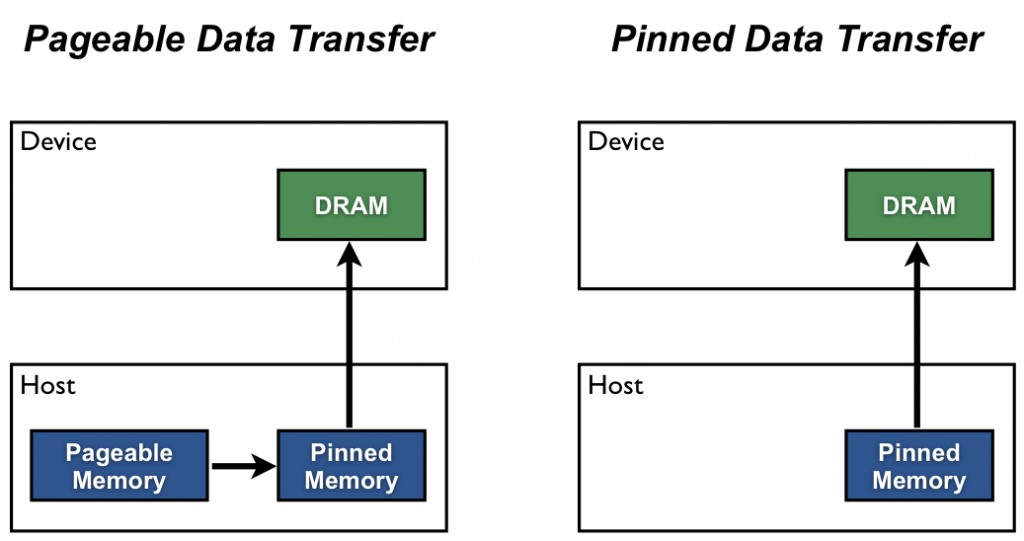
\includegraphics[width = \linewidth]{figures/datatransfer}
	\caption{The difference between copying pinned and pageable memory~\cite{nvidia_how_2012}}
 	\label{fig:memcopy}
 \end{figure}
 
 \subsubsection{Device Memory}
 \label{sec:devMem}
 Device memory, in this case, is defined as the RAM found locally on the graphics card, also known as Video RAM (VRAM). It is not accessible to CPU code and data must first be copied into the device memory for the GPU to execute operations on said data. The CUDA API offers the method shown in Figure \ref{fig:cudamalloc} to allocate memory on the device~\cite{nvidia_cuda_2022-1}.
 
 The method has similar parameters to the CUDA method described in section \ref{sec:hostMem}, with $devPtr$ being the equivalent to $ptr$. 
 
 \begin{figure}[htpb]
 	\centering
 	\begin{tabular}{c}
 		\begin{lstlisting}[language=C++]
 			cudaError_t cudaMalloc(void** devPtr, size_t size);
 		\end{lstlisting}
 	\end{tabular}
 	\caption[CUDA device memory allocation]{The CUDA method to allocate device memory~\cite{nvidia_cuda_2022-1}}
 	\label{fig:cudamalloc}
 \end{figure}

 
 \subsubsection{Managed Memory}
 \label{sec:manMem}
 Unified memory, also known as managed memory, is a technique used by CUDA to enable both CPU and GPU to access the same address space. However, it is more of a software feature than hardware allowing the GPU to access CPU memory space or vice-versa, as the data in question will always be moved to the executing processor's address space before operations are performed on said data~\cite{nvidia_unified_2017}. Figure \ref{fig:mallocmanaged} shows the method required to allocate managed memory~\cite{nvidia_cuda_2022-1}.
 
 Similar to the other CUDA allocates, an explanation to the parameters $devPtr$, again equivalent to $ptr$, and $size$ can be found in section \ref{sec:hostMem}. The parameter $flags$ indicates the access permissions for the chunk of memory, defaulting to accessible by any stream from any device~\cite{nvidia_cuda_2022-1}.
  
  \begin{figure}[htpb]
 	\centering
 	\begin{tabular}{c}
 		\begin{lstlisting}[language=C++]
 			cudaError_t cudaMallocManaged(void** devPtr, size_t size, 
 				unsigned int flags = cudaMemAttachGlobal);
 		\end{lstlisting}
 	\end{tabular}
 	\caption[CUDA managed memory allocation]{The CUDA method to allocate managed memory~\cite{nvidia_cuda_2022-1}}
 	\label{fig:mallocmanaged}
 \end{figure}
 
 
 \subsubsection{Memory Copy}
 
 CUDA uses one method to copy memory both to and from the device memory, which can be seen in Figure \ref{fig:cudamemcpy}. The method copies $count$ bytes of memory from the pointer $src$ to the location $dst$ points to. The enum $cudaMemcpyKind$ defines the type of memory transfer it is. The copy types supported are~\cite{nvidia_cuda_2022-1}:
 
 \begin{itemize}
 	\item cudaMemcpyHostToHost
 	\item cudaMemcpyHostToDevice
 	\item cudaMemcpyDeviceToHost
 	\item cudaMemcpyDeviceToDevice
 	\item cudaMemCpyDefault: this is the recommended 'kind', as this causes the method to infer the type of transfer from the pointer values~\cite{nvidia_cuda_2022-1}.
 \end{itemize}
 
  \begin{figure}[htpb]
 	\centering
 	\begin{tabular}{c}
 		\begin{lstlisting}[language=C++]
 			cudaError_t cudaMemcpy(void* dst, const void* src, 
 				size_t count, cudaMemcpyKind kind);
 		\end{lstlisting}
 	\end{tabular}
 	\caption[CUDA memory copy]{The CUDA method to copy memory~\cite{nvidia_cuda_2022-1}}
 	\label{fig:cudamemcpy}
 \end{figure}
 
 
 \subsection{NVML}
 
 Nvidia Management Library, abbreviated NVML, is a part of the CUDA API that offers, as its name suggests, management and monitoring capabilities. NVML can monitor many aspects of the GPU, such as GPU utilization, currently active processes, the current performance state of the GPU, and more~\cite{nvidia_nvidia_2011}. Delving deeper into the documentation to NVML, it is revealed that the library is also able to monitor some aspects of the PCIe link that connects the GPU to the CPU. Supported metrics are the throughput and basic information about the PCIe link~\cite{nvidia_device_2021}. Figure \ref{fig:nvmlpcie} shows the method call required to query the library about the PCIe throughput. The $device$ parameter is the identifier of the GPU, and $counter$ defines the counter type. Supported counter types are~\cite{nvidia_device_2021}: 
 \begin{itemize}
 	\item NVML\_PCIE\_UTIL\_TX\_BYTES
 	\item NVML\_PCIE\_UTIL\_RX\_BYTES
 	\item NVML\_PCIE\_UTIL\_COUNT
 \end{itemize}
Whilst the documentation does not specify in further detail what each counter means, it can be inferred that TX means transmit and RX means receive, as TX and RX are common abbreviations for transmitter and receiver. [does this need citing? if so cite the book and change wording] Finally, the last parameter $value$ points to the location where the counter value will be written to~\cite{nvidia_device_2021}.

   \begin{figure}[htpb]
 	\centering
 	\begin{tabular}{c}
 		\begin{lstlisting}[language=C++]
 			nvmlReturn_t nvmlDeviceGetPcieThroughput ( nvmlDevice_t device,
 				nvmlPcieUtilCounter_t counter, unsigned int* value );
 		\end{lstlisting}
 	\end{tabular}
 	\caption[NVML counter readout]{The NVML method read the PCIe link throughput~\cite{nvidia_cuda_2022-1}}
 	\label{fig:nvmlpcie}
 \end{figure}
 
 [that should be everything, de-allocation maybe?]

 
 
\section{PCI-Express}
The last section mentioned the ability to move data from the main memory to the device memory, and vice-versa. This is done, on a lower level, by PCI-Express. 

PCIe, or PCI-Express, shorthand for Peripheral Component Interconnect Express, is a "general-purpose serial I/O interconnect"~\cite{pci-sig_pci_2011}. PCIe, as an interface, allows the CPU to connect with, as the name suggests, peripherals and components. Common components and peripherals include, but are not limited to: Graphics cards, sound cards, video capture cards, WiFi cards, and storage.

PCIe is designed to replace the ageing PCI (Peripheral Component Interconnect), PCI-X (Peripheral Component Interconnect Extended), and AGP (Accelerated Graphics Port) standards~\cite{verma_pcie_2017}. These standards are developed, defined, and maintained by the PCI-SIG group, which is a nonprofit organization with 800+ member companies based in Beaverton, Oregon~\cite{pci-sig_contact_2022}. This section will briefly introduce the key features and functionality of PCI-Express.

\subsection{Key Features}

PCI-Express is, at its core, a serialized, point-to-point connection that is designed to be processor agnostic, scalable, and backwards compatible with PCI~\cite{lawley_understanding_2014, pci-sig_pci_2011, pci-sig_membership_2022}. PCI-Express utilizes a dual-simplex connection to facilitate sending and receiving information concurrently. Additionally, to ensure backwards compatibility with PCI, PCI-Express shares the same memory configuration as PCI, which will be elaborated further upon in section \ref{sec:memory}. Further key features include improvements in error handling and data integrity~\cite{verma_pcie_2017}. To future-proof the standard, current and future generations of PCIe are to be designed to be compatible with current PCIe standards~\cite{pci-sig_membership_2022}. So far, each generation of PCIe doubled the previous generation's theoretical maximum bandwidth, as seen in Table \ref{tab:bandwidths}.

[todo: gen4 bandwidths, mention gen4 as SOTA]

\begin{table}[htpb]
\includegraphics[width = \linewidth]{figures/PCIE-bandwidths}
\caption{PCI Express aggregate bandwidths by generation and link width ~\cite{jackson_pci_2012}}
\label{tab:bandwidths}
\end{table}

\subsection{Functionality}

\subsubsection{packet}
PCIe, similar to IPv4 or IPv6, utilizes packets to communicate between the host - the CPU - and the device. As shown in Figure \ref{fig:packet}, the packet consists of a few different elements, which will be further expanded upon below. Additionally, PCIe communication is separated into three primary layers, with each being responsible for a specific set of functions. The Physical layer is responsible for translating the packets to electrical signals and vice-versa. The Data Link Layer is primarily responsible for link error detection and correction. The Transaction layer is primarily responsible for flow control and transaction ordering~\cite{lawley_understanding_2014}.

\begin{figure}[htpb]
\includegraphics[width = \linewidth]{figures/PCIE-packet}
\caption{An example of a PCI-Express packet ~\cite{lawley_understanding_2014}}
\label{fig:packet}
\end{figure}

\begin{itemize}
\item Start: this is the start component which signals the begin of a packet to the Physical layer.
\item Sequence: This two-byte sequence is used by the Data Link Layer to determine the sequence of the packets and to ensure that no packets have gone missing.
\item Header: The 12 to 16 Byte header will be discussed in further detail in subsection \ref{sec:header}. This component belongs to the Transaction layer. 
\item Payload: The PCIe payload. This is optional, however any memory transferred via memory copy operations will have the memory as payload. This also is a part of the Transaction layer.
\item ECRC: a CRC code for error-checking purposes used by the Transaction layer.
\item LCRC: a CRC code for error-checking purposes used by the Data Link Layer.
\end{itemize}

[question: do i need a source for each of the bullet points? additionally, the source doesn't outright state that 'this is what this is for', in a degree, but it is inferred knowledge. what should I do about this?]

\subsubsection{header}
\label{sec:header}
As with IPv4 or IPv6, PCI-Express uses headers to determine the purpose and target of each TLP (Transaction Layer Packet).
However, instead of using IP-addresses, stored in the header, to determine the sender and the receiver, PCIe uses the Requester ID to determine the sender. The Address determines the receiver of the intended packet, as the device memory is memory-mapped into the host address domain to enable the processor's native load or store instructions to work with PCIe devices~\cite{oracle_inc_pci_2010}. As seen in Figure \ref{fig:header}, the header has a fixed format, similar to an IPv4 or v6 header. The fields and their uses are briefly explained below.

[todo: example IPv4/v6 header]

\begin{figure}[htpb]
\includegraphics[width = \linewidth]{figures/PCIE-header}
\caption{An example of a memory request header ~\cite{lawley_understanding_2014}}
\label{fig:header}
\end{figure}

\begin{itemize}
\item TC: Traffic Class: this denotes the priority of the packet. A larger value represents a higher priority.~\cite{jackson_pci_2012}
\item TD: The TLP Digest field. If TD is set to 1, it indicates that there is additional CRC data in the TLP data. [cite xillybus]
\item Length: more or less self-explanatory: length denotes the length of the payload in Double Words. [cite xillybus]
\item Requester ID: self-explanatory: the ID of the device that requested or sent the packet. [cite xillybus]
\item Tag: The Tag field has the function of a tracking number, as for read requests, the device must copy this value to its response. All outstanding tags must be unique to ensure data integrity. Some request types, such as write requests, do not utilize tags. [cite xillybus]
\item DW BE fields: DW BE stands for Double-Word Byte Enable. This denotes which of the bytes in the first / last DWs are valid. [cite xillybus]
\item Address: self-explanatory: The Address to which this packet is addressed, as explained above. Additionally, for read and write requests, this denotes the starting address of the read or write. [cite xillybus]
\item The EP and Attr fields are not further elaborated upon as they are rarely used by PCIe endpoint devices. [cite xillybus]
\end{itemize}

[todo: update and verify with book]

\subsection{Topology and Communication}

\subsubsection{Topology}
There are four significant components to be mentioned when discussing the topology of a PCI-Express based system. PCIe endpoints, switches, bridges, and a root complex. 
The communication between CPU cores and memory controllers to the PCIe endpoint is handled by the PCIe root complex. This communication can be routed through (but does not require) PCIe switches. PCIe switches allow for cascading connections, however do not benefit the total bandwidth, which is limited by the PCIe root complex in a CPU~\cite{nakamura_thorough_2017}.
Bridges are used to connect legacy PCI and PCI-X devices with the PCIe root complex~\cite{pci-sig_pci_2011}.
Figure \ref{fig:topology} shows an example PCIe configuration of an Intel-based processor.

\begin{figure}[htpb]
\includegraphics[width = \linewidth]{figures/PCIE-topology}
\caption{PCIe configuration on an Intel-based system~\cite{nakamura_thorough_2017}}
\label{fig:topology}
\end{figure}

\subsubsection{Memory Management}
\label{sec:memory}

Each PCI-Express device has some built-in storage and registers to facilitate communication between the device and the rest of the system. This memory is, due to compatibility reasons, structured in the same way as the structure found in the older PCI standard. This divides the PCIe device memory into three major parts for addressing and memory access~\cite{jackson_pci_2012}:

\begin{itemize}
\item Configuration
\item Memory
\item IO
\end{itemize}

The configuration address space enables software to both identify and correctly configure the device, and is defined by its physical bus and device number~\cite{oracle_inc_pci_2010}. It also enables the software to control and check the status of a PCIe device~\cite{jackson_pci_2012}.

The memory address space is where the internal storage of a PCIe device is mapped~\cite{jackson_pci_2012}. This memory space is also memory-mapped to the CPU's address domain for ease of access by the CPU~\cite{oracle_inc_pci_2010}.

The IO address space is a place dedicated to accessing the internal registers / storage of a PCIe or PCI device. However, this is mostly deprecated in PCIe as the internal registers and storage of said devices are simply mapped into the memory address space instead. It is now common practice to map the same set of registers in both memory and IO address space for backwards compatibility purposes. The PCIe specification discourages use of the IO space, which indicates that it remains solely for legacy support purposes~\cite{jackson_pci_2012}.

\subsubsection{Links and Lanes}
A connection between the two PCIe devices is called a link, which is made up of lanes~\cite{jackson_pci_2012}. A PCIe device, in this case, can be the CPU's PCIe root complex, bridges, switches, or a PCIe end point. A lane, on the hardware level, is a set of four copper wires, two for each signal direction~\cite{jackson_pci_2012}. Due to the scalability of PCIe, the amount of lanes in a link is variable, from 1 up to 32, and is represented by a x in front of the lane width, e.g. PCIe x16, which indicates that the PCIe link has 16 lanes. A wider link means higher bandwidths and transmit capabilities, however it also means higher power consumption, space, and cost~\cite{jackson_pci_2012}. Figure \ref{fig:link} illustrates an example PCIe link with several lanes. A normal GPU will usually have a PCIe x16 link.


\begin{figure}[htpb]
\begin{center}
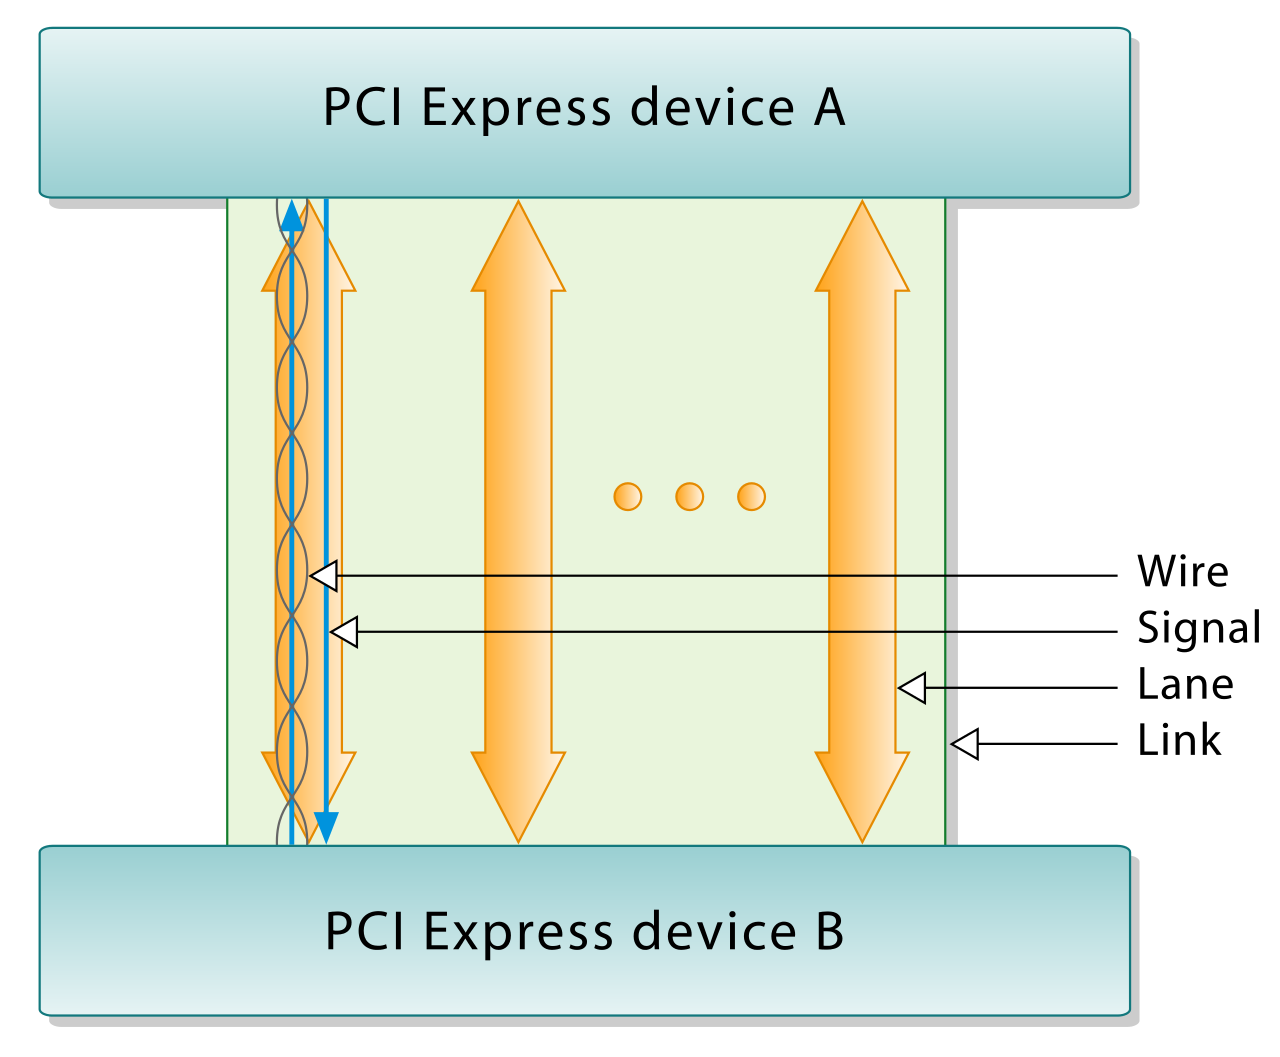
\includegraphics[height = 200px]{figures/PCIE-link}
\caption{An example PCIe link between two devices~\cite{budruk_pci_2014}}
\label{fig:link}
\end{center}
\end{figure}

\subsection{Revisions and Further Specifications}

PCI-Express was first introduced in 2003, and has received a new revision once every three to four years on average. Whilst most current hardware uses PCIe 3.0 and 4.0, introduced in 2010 and 2017 respectively~\cite{sharma_pci_2020}, PCI-SIG has already published their specifications for the PCIe 5.0 and 6.0 standards. These, again, double the bandwidths of the previous generation, enabling theoretical transfer speeds of up to 128GB/sec in both directions on a PCIe 6.0 x16 link~\cite{sharma_pci_2020}. However, it is to be expected that these high-speed interconnect standards will take a few years to become widely available and adopted, as Intel only released their first PCIe 5.0-capable CPUs around the end of 2021~\cite{intel_product_2022}. 

Additionally, other manufacturers and companies have developed their own protocols and standards to extend the feature-set of PCIe, such as Intel's Thunderbolt, which enables PCIe devices to be connected externally with only a small loss of performance~\cite{intel_what_2022-1}. Another example is the NVMe standard, a PCIe-compatible interface specifically devised and optimized for high-bandwidth, low-latency storage solutions~\cite{kingston_understanding_2017}.





